\documentclass[12pt]{article}
\usepackage{times}
\usepackage{indentfirst}

\usepackage[a4paper,left=1.5in,right=1in,top=0.5in,bottom=1in,nohead]{geometry}
%%%%%%%%%%%%% For the image in report
\usepackage{graphicx}
\usepackage{float}
%%%%%%%%%%%%%%
\usepackage{mathtools}
\usepackage{amsmath}
% for justify alignment
\usepackage{ragged2e}
\usepackage{titlesec}
\usepackage{standalone}
\usepackage{times}
%%\usepackage[T1]{fontenc} % not working in my report font
\usepackage{mathptmx}
%%%%%%%%%%%%%%%%%% Remove dotted line from list of content
\makeatletter
\renewcommand{\@dotsep}{10000}
\makeatother
%%%%%%%%%%%%%%%%%%


\setcounter{secnumdepth}{5}

\begin{document}


%% this if list of contents
\tableofcontents
\thispagestyle{empty}
\cleardoublepage
% this is list of figure
\listoffigures
\thispagestyle{empty}
\cleardoublepage
%%%%%%%%%%%%%%%%%%%
\listoftables
\thispagestyle{empty}
\cleardoublepage

%%%%%%%%%%% Add list of Figure and Synopsis
\addcontentsline{toc}{section}{\numberline{} List of Figure}
\addcontentsline{toc}{section}{\numberline{} List of Table}
\addcontentsline{toc}{section}{\numberline{} SYNOPSIS}
%%%%%%%%%%%

\section*{SYNOPSIS}
	\justify
	The telecommunication always tries to reach the best performances, the reliability and the efficiency with the lowest possible costs. In this domain, antennas establish a basic element allowing the transmission of the electromagnetic waves in free space. We find several types of antennas which different by cuts, geometrical shape, capacity of transmission. The most serious limitations of the microstrip antenna is its narrow band, which is typically of the order of some percents 1-5 \%. However, the new generation of the communication, the mobile or satellite communication, provokes considerable changes in patches antennas, from which the various modern applications require a functioning in wideband.
	This  project will design and analyze a rectangular Microstrip patch antenna by using the software HFSS.Microstrip antennas have a profile which relays at the needs of new technology, such as a low profile, a flat configuration and a better gain. The simple configuration of the rectangular microstrip antenna presents generally a narrow band. The project will take effort to enhance gain and bandwidth with inclusion of symmetrical shape slots placed on the patch surface.
\thispagestyle{empty}
\cleardoublepage





\setcounter{page}{1}
% This is the Introduction to my project
\section{Introduction}\label{sec:Introduction}
% This is the objective, need and organiztion


\subsection{Objective}\label{subs:Objective}
 \justify
   A  rectangular microstrip antenna is a type of radio antenna with a low profile, which can be mounted on a flat surface. It consists of a flat rectangular sheet of metal, mounted over a larger sheet of metal called a ground plane.The two metal sheets together form a resonant piece of microstrip transmission line with a length of approximately one-half wavelength of the radio waves. The radiation mechanism arises from discontinuities at each truncated edge of the microstrip transmission line.These patch antennas are used as simple and for the widest and most demanding applications. Dual characteristics, circular polarizations, dual frequency operation, frequency agility, broad band width, feed line flexibility and beam scanning can be easily obtained from these patch antennas.

 \justify
  Rectangular Microstrip Patch Antenna with High Gain for 3.1 GHz - 10.6 GHz Applications development of low cost, minimal weight and low profile antennas that are capable of maintaining high performance over a wide spectrum of frequencies. This technological trend has focused much effort into the design of a microstrip patch antenna. The objective of this paper is to design, and fabricate an inset fed rectangular microstrip patch antenna.

\subsection{Need}\label{sub:Need}
 \justify
   Microstrip patch antennas are increasing in popularity for use in wireless applications due to their low-profile structure. Therefore they are extremely compatible for embedded antennas in handheld wireless devices such as cellular phones, pagers etc... The telemetry and Square Rectangular Dipole Circular Triangular Circular Ring Elliptical communication antennas on missiles need to be thin and conformal and are often Microstrip patch antennas. Another area where they have been used successfully is in Satellite communication.

 \justify
   Microstrip patch antennas have a very high antenna quality factor (Q). Q represents the losses associated with the antenna and a large Q leads to narrow bandwidth and low efficiency. Q can be reduced by increasing the thickness of the dielectric substrate.

 \justify
   As per requirement many new shapes can replace the conventional shapes .There are many shapes in the field of microstrip patch antenna .A design of slots on the patch and making defected structure in the ground plane for improving the bandwidth as well as achieving the multiband operation which is the part of this project is very good for future aspects. All works has been performed in the thesis with the HFSS simulation software.

\cleardoublepage


\subsection{Organisation}\label{sub:Organisation}
 \justify
  \textbf{Chapter 1}

      It contains the overall introduction to the rectangular microstrip patch antenna.In this chapter also concluded with the details of outline of the present report .\
 \justify
  \textbf{Chapter 2}

      It is dedicated to literature survey which gives an overview about microstrip patch antenna based on various international publish papers on IEEE, google scholar etc.
 \justify
  \textbf{Chapter 3}

      It is based on totally system modeling i.e. total description of technical parts related to topic.The basic parameters on which the selection and performance of an Antenna is characterize are bandwidth, Antenna polarization, Radiation , Beamwidth ,Pattern, Directivity, efficiency etc are described. All the popular feeding methods used in microstrip antenna with their significance are also discussed.
 \justify
  \textbf{Chapter 4}

      It contains Advantages and Applications of Microstrip Patch Antenna.
 \justify
  \textbf{Chapter 5}

      It contains the conclusion of the project report.
\cleardoublepage
% this is literature survey
\section{Literature Survey}\label{sec:Literature Survey}
\justify
	The paper studies the method of using a ground slot for bandwidth improvement of compact ultra-wide band (UWB) antennas 	with microstrip line feed. Slots of different shapes such as triangular, rectangular, partially circular and hexagonal, placed on the ground plane under the feed line of the radiator are studied for impedance matching. \\

	
	\begin{flushleft}
		\textbf{Paper 1}
	\end{flushleft}

	\begin{center}
		   \begin{table}[h]

		   	\begin{tabular}{ |l|p{11cm}| }
		   		\hline
		   		Title of paper &  Bandwidth Improvements Using Ground Slots for Compact UWB Microstrip-fed Antennas \\
		   		\hline
		   		Authors & L. Liu, S. W. Cheung, and T. I. Yuk \\
		   		\hline
		   		Year of Publication & 2011 \\
		   		\hline
		   		Publishing details & International Conference on Education Technology and Computer (IEEE) \\ \hline
		   		Summary & A small microstip-fed monopole antenna, which consists of a rectangular patch and a truncated ground plane, is presented for ultra wideband application. The proposed antenna is designed to operate over 3.1 to 11 GHz for 11 10 dB. Good return loss and radiation pattern characteristics are obtained in the frequency band of interest.\\
		   		\hline
		   		Weblink & http://ieeexplore.ieee.org/stamp/stamp.jsp?tp=arnumber=5403292 \\
		   		\hline
		   	\end{tabular}

		   \end{table}
	\end{center}

	\begin{flushleft}
		\textbf{Paper 2}
	\end{flushleft}


	 \begin{center}
	 	\begin{table}[h]
	 		\centering
	 		\begin{tabular}{ |l|p{11cm}| }
	 			\hline
	 			Title of paper &  Planar UWB antenna with multi-slotted ground plane \\
	 			\hline
	 			Authors & Azim, R., M. T. Islam, N. Misran, S. W. Cheung, and Y. Yamada \\
	 			\hline
	 			Year of Publication & 2011 \\
	 			\hline
	 			Publishing details & The paper studies the method of using a ground slot for bandwidth improvement of compact ultra-wide band (UWB) antennas with microstrip line feed. Slots of different shapes such as triangular, rectangular, partially circular and hexagonal, placed on the ground plane under the feed line of the radiator are studied for impedance matching.\\
	 			\hline
	 			Weblink & http://ieeexplore.ieee.org/stamp/stamp.jsp?tp=arnumber=5403292 \\
	 			\hline
	 		\end{tabular}

	 	\end{table}
	 \end{center}

	\cleardoublepage
	
		\begin{flushleft}
			\textbf{Paper 3}
		\end{flushleft}
		

	  \begin{center}
	  	\begin{table}[h]
	  		\centering
	  		\begin{tabular}{ |l|p{11cm}| }
	  			\hline
	  			Title of paper &  Printed band-rejection UWB antenna with H-shaped slot \\
	  			\hline
	  			Authors & Bao, X. L. and M. J. Ammann \\
	  			\hline
	  			Year of Publication & 2012 \\
	  			\hline
	  			Publishing details & The ground element of the proposed antenna is taken in the form of defected ground structure. The antenna is fed by a microstrip feeding technique and printed on a dielectric Fr4 substrate of dimension (30mm X 32 mm) permittivity εr =4.4 and height h = 1.59 mm. The optimization on the microstrip has been done to accomplish an -10 dB return loss criterion. Design parameters like substrate variation, feed size and defected ground plane which affect the performance of the antenna in terms of its frequency domain and time domain characteristics are investigated.\\
	  			\hline
	  			Weblink & http://ieeexplore.ieee.org/stamp/stamp.jsp?tp=arnumber=5403292 \\
	  			\hline
	  		\end{tabular}

	  	\end{table}
	  \end{center}

	\begin{flushleft}
		\textbf{Paper 4}
	\end{flushleft}


		   	\begin{table}[h]
		   		\centering
		   		\begin{tabular}{ |l|p{11cm}| }
		   			\hline
		   			Title of paper &  Inverted triangle printed monopole antenna with halfdisk for UWB applications \\
		   			\hline
		   			Authors & Chayono, R., M. Haneishi, and Y. Kimura \\
		   			\hline
		   			Year of Publication & 2013 \\
		   			\hline
		   			Publishing details & International Conference on Education Technology and Computer (IEEE) \\ \hline
		   			Summary & A small microstip-fed monopole antenna, which consists of a rectangular patch and a truncated ground plane, is presented for ultra wideband application. The proposed antenna is designed to operate over 3.1 to 11 GHz for 11 10 dB. Good return loss and radiation pattern characteristics are obtained in the frequency band of interest.\\
		   			\hline
		   			Weblink & http://ieeexplore.ieee.org/stamp/stamp.jsp?tp=arnumber=5403292 \\
		   			\hline
		   		\end{tabular}

		   	\end{table}

  	  \cleardoublepage
  	  
		\begin{flushleft}
			\textbf{Paper 5}
		\end{flushleft}


	    	\begin{table}[h]
	    		\centering
	    		\begin{tabular}{ |l|p{11cm}| }
	    			\hline
	    			Title of paper & Small modified monopole antenna for UWB application \\
	    			\hline
	    			Authors & Ojaroudi, M., G. Kohneshahri, and J. Noory \\
	    			\hline
	    			Year of Publication & 2013 \\
	    			\hline
	    			Publishing details & International Conference on Education Technology and Computer (IEEE) \\ \hline
	    			Summary & A two-port rectangular microstrip patch antenna for dual frequency operation is investigated in this paper. Simple microstrip line feed has been used to feed the antenna. Quarter wavelength transformer is used for impedance matching. For the conventional dual feed dual frequency antenna the isolation between the two ports is obtained as 30 dB. An Improvement in isolation performance has been achieved by the introduction of defected microstrip structure which acts as band stop filters and thereby increases isolation between the two ports.\\
	    			\hline
	    			Weblink & http://ieeexplore.ieee.org/stamp/stamp.jsp?tp=arnumber=5403292 \\
	    			\hline
	    		\end{tabular}

	    	\end{table}
	    	
	    	\begin{flushleft}
	    		\textbf{Paper 6}
	    	\end{flushleft}
	    	

		  \begin{center}
		  	\begin{table}[H]
		  		\centering
		  		\begin{tabular}{ |l|p{11cm}| }
		  			\hline
		  			Title of paper &  Development of a practical ultra- wideband antenna with planar circuit integration possibilities \\
		  			\hline
		  			Authors & G. Brzezina , Q. Ye , L. Roy \\
		  			\hline
		  			Year of Publication & 2013 \\
		  			\hline
		  			Publishing details & International Conference on Education Technology and Computer (IEEE) \\ \hline
		  			Summary & The printed antenna is one of the best antenna structures, due to its low cost and compact design. In this paper a new approach to improve the radiation effectiveness and the performance of antennas by miniaturization of the size. Indeed, we have studied the performance of ultra wideband antenna which consists of a ring-shaped patch. This study was made for the whole frequency band of UWB ranging from 2.5GHz to 9.4GHz and the geometry of the antenna and the results were obtained using the simulation software. \\
		  			\hline
		  			Weblink & http://ieeexplore.ieee.org/stamp/stamp.jsp?tp=arnumber=5403292 \\
		  			\hline			 
		  		\end{tabular}		
		  		
		  	\end{table}
		  \end{center}
		  
		\cleardoublepage
			
			\begin{flushleft}
				\textbf{Paper 7}
			\end{flushleft}
			

		  \begin{center}
		  	\begin{table}[H]
		  		\centering
		  		\begin{tabular}{ |l|p{11cm}| }
		  			\hline
		  			Title of paper & Comparison between Straight and U shape of ultra-wideband microstrip antenna using log periodic technique  \\
		  			\hline
		  			Authors & M. K. A. Rahim, M. N. A. Karim, T. Masri, A. Asrokin \\
		  			\hline
		  			Year of Publication & 2013 \\
		  			\hline
		  			Publishing details & International Conference on Education Technology and Computer (IEEE) \\ \hline
		  			Summary & A band notched ultra-wideband (UWB) patch antenna is presented with its circuit modeling. The rectangular patch antenna is designed on dielectric substrate and fed with 50 Ω microstrip by optimizing the width of partial ground, the width of the feed line to operate in UWB. This antenna consists of a radiating element with a strip, and a partial ground plane and feeding line has been demonstrated. With the design, the return loss is lower than 10 dB in 3.1-10.6 GHz frequency range and show the band-notch characteristic in the UWB band to avoid interferences, which is caused by WLAN (5.15–5.825 GHz) and WiMax (5.25–5.85 GHz) systems. \\
		  			\hline
		  			Weblink & http://ieeexplore.ieee.org/stamp/stamp.jsp?tp=arnumber=5403292 \\
		  			\hline			 
		  		\end{tabular}		
		  		
		  	\end{table}
		  \end{center} 
				 
			\begin{flushleft}
				\textbf{Paper 8}
			\end{flushleft}
			

		  \begin{center}
		  	\begin{table}[H]
		  		\centering
		  		\begin{tabular}{ |l|p{11cm}| }
		  			\hline
		  			Title of paper &  Wide band high efficiency printed loop antenna design for wireless communication systems  \\
		  			\hline
		  			Authors & Denidni, T.A., L., Lim, Y., and Rao, Q \\
		  			\hline
		  			Year of Publication & 2014 \\
		  			\hline
		  			Publishing details & International Conference on Education Technology and Computer (IEEE) \\ \hline
		  			Summary & A fractal monopole antenna is proposed for the application in the UWB frequency range, which is designed by the combination of two fractal geometries.A fractal micro strip antenna is used for multiband application in this project provides a simple and efficient method for obtaining the compactness. A sierpinski carpet based fractal antenna is designed for multiband applications. It should be in compactness and less weight is the major point for designing an antenna. This antenna is providing better efficiency.\\
		  			\hline
		  			Weblink & http://ieeexplore.ieee.org/stamp/stamp.jsp?tp=arnumber=5403292 \\
		  			\hline			 
		  		\end{tabular}		
		  		
		  	\end{table}
		  \end{center}
		
		\cleardoublepage
		
			\begin{flushleft}
				\textbf{Paper 9}
			\end{flushleft}
			
	
		  \begin{center}
		  	\begin{table}[H]
		  		\centering
		  		\begin{tabular}{ |l|p{11cm}| }
		  			\hline
		  			Title of paper &  Design of reconfigurable slot antenna  \\
		  			\hline
		  			Authors & Peroulis, D., Sarabi, K., and Katehi, L.P.B \\
		  			\hline
		  			Year of Publication & 2014 \\
		  			\hline
		  			Publishing details & The characteristics of a small antenna using an H-shaped microstrip patch antenna are analyzed. Operating frequency of H-shaped microsrip antenna is 2 GHz. The theoretical results are compared with experimental result using cavity model. Comparison with other reported results justify the veracity of the proposed method. Significant reduction of antenna size can be realized when the H-shaped patch is used instead of the conventional rectangular microstrip patch antenna. This antenna is providing better efficiency.\\
		  			\hline
		  			Weblink & http://ieeexplore.ieee.org/stamp/stamp.jsp?tp=arnumber=5403292 \\
		  			\hline			 
		  		\end{tabular}		
		  		
		  	\end{table}
		  \end{center}
		  
			 	\begin{flushleft}
			 		\textbf{Paper 10}
			 	\end{flushleft}
			 	
		 
		 
		    \begin{center}
		    	\begin{table}[H]
		    		\centering
		    		\begin{tabular}{ |l|p{11cm}| }
		    			\hline
		    			Title of paper &  Design of band notched UWB patch antenna with circular slot  \\
		    			\hline
		    			Authors & Shilpa Jangid and Mithilesh Kumar \\
		    			\hline
		    			Year of Publication & 2011 \\
		    			\hline
		    			Publishing details & Different feeding techniques of microstrip patch antennas with different spiral defected ground structures are presented in this paper. The investigated structures illustrate some merits in designing multi-electromagnetic band-gap structures by adjusting the capacitance and changing the inductance through varying the width and length of spiral defected ground structure.\\
		    			\hline
		    			Weblink & http://ieeexplore.ieee.org/stamp/stamp.jsp?tp=arnumber=5403292 \\
		    			\hline			 
		    		\end{tabular}		
		    		
		    	\end{table}
		    \end{center}
		    
		    \cleardoublepage
		    
		    	\begin{flushleft}
		    		\textbf{Paper 11}
		    	\end{flushleft}
		    	

		      \begin{center}
		      	\begin{table}[H]
		      		\centering
		      		\begin{tabular}{ |l|p{11cm}| }
		      			\hline
		      			Title of paper &  Microstrip Antenna gain enhancement using left-handed metamaterial structure \\
		      			\hline
		      			Authors & H.A. Majid, M.K.A. Rahim and T. Marsi \\
		      			\hline
		      			Year of Publication & 2015 \\
		      			\hline
		      			Publishing details & International Conference on Education Technology and Computer (IEEE) \\ \hline
		      			Summary & This paper describes the effect of temperature variation on microstrip patch antenna for different substrate materials. Eight materials are chosen as substrate and the effect of temperature variation is studied on each substrate material. A technique of temperature compensation has also been developed with substrate height variation. It is also seen that the change in resonance frequency due to variation of temperature can be compensated by varying the height of the substrate. The proposed antenna is designed and simulated by using HFSS software.\\
		      			\hline
		      			Weblink & http://ieeexplore.ieee.org/stamp/stamp.jsp?tp=arnumber=5403292 \\
		      			\hline			 
		      		\end{tabular}		
		      		
		      	\end{table}
		      \end{center}
		      
		      	\begin{flushleft}
		      		\textbf{Paper 12}
		      	\end{flushleft}
		      	

		       \begin{center}
		       	\begin{table}[H]
		       		\centering
		       		\begin{tabular}{ |l|p{11cm}| }
		       			\hline
		       			Title of paper &  Single-feed dual-frequency rectangular microstrip antenna with square slot \\
		       			\hline
		       			Authors & Chen W. S. \\
		       			\hline
		       			Year of Publication & 2015 \\
		       			\hline
		       			Publishing details & International Conference on Education Technology and Computer (IEEE) \\ \hline
		       			Summary & This paper presents the result for antenna factor of microstrip patch antenna when used as electromagnetic interference (EMI) sensor. Antenna factor is an important parameter of a sensor used for EMI measurements. The microstrip antenna has found wide application as transmit and receive antenna in modern microwave systems. In this paper, a new application of microstrip antenna as EMI sensor is presented. The result for antenna factor versus frequency of a microstrip patch antenna is presented using commercial software CST Microwave Studio. Also the experimental results for a prototype antenna are presented and compared with the simulated result.\\
		       			\hline
		       			Weblink & http://ieeexplore.ieee.org/stamp/stamp.jsp?tp=arnumber=5403292 \\
		       			\hline			 
		       		\end{tabular}		
		       		
		       	\end{table}
		       \end{center}		 
		
		\cleardoublepage
		
			\begin{flushleft}
				\textbf{Comparision}
			\end{flushleft}
			

		\begin{center}
			\begin{table}[H]
				\begin{tabular}{ |p{8cm}|p{7cm}|}
					\hline
					PAPER & RESULT \\ \hline
					
					Bandwidth Improvements Using Ground Slots for Compact UWB Microstrip-fed Antennas & The hexagonal slot provides the largest impedance bandwidth of 3.1-16.3 GHz for S11 < ¡10 dB, with an average gain of about 2.8 dBi and an average efficiency of about 88\% \\ \hline
					
					Development of a practical ultra- wideband antenna with planar circuit integration possibilities & This antenna can also be operated at 2.478 GHz as it provides dual band operation. At 2.478 GHz the values of Return loss and bandwidth are -30.218dB and 33.1 MHz respectively \\ \hline
					
					Wide band high efficiency printed loop antenna design for wireless communication systems & A compact, 31mm x 21mm low profile planar ultra-wide band patch antenna was introduced. The antenna was ex-cited using a rectangular edge-feed microstrip feed line. The impedance bandwidth of the antenna is about 11 GHz (3.0-14GHz), which exceeds the FCC UBW requirement. \\ \hline
					
					Design of reconfigurable slot antenna & Besides exhibiting a 10-dB bandwidth of 172\% with 13.06:1 ratio bandwidth, a 14-dB bandwidth (low return loss) of 79\% is also demonstrated in the higher UWB operating bands for outdoor propagation.\\ \hline
					
					Design of band notched UWB patch antenna with circular slot  & The patch antenna ring ultrawide-bandwidth radiating between 2.5GHz and 9.4GHz in order to achieve the
					operation Bluetooth / ISM, 2.5/3.5 GHz and 5.2/5.7 GHz WiMAX WLAN. \\ \hline
					
					Microstrip Antenna gain enhancement using left-handed metamaterial structure & The resonant frequency of the antenna is 1.99 GHz.
					return loss with frequency of antenna is found to be -30.33 dB at resonant frequency 1.99 GHz. \\ \hline
					
					Single-feed dual-frequency rectangular microstrip antenna with square slot &  At 2GHz the verified and tested result on RadiationEfficiency=91.99\%, Directivity=5.4dBi,Directive gain=4.98dBi \\ \hline
					
					
					
				\end{tabular}
			\end{table}
		\end{center}


\cleardoublepage

\section{System Modeling}\label{sec:System Modeling}
 \subsection{Property of Basic Antenna}\label{sub:Property of Basic Antenna}
	  \justify
	   A Microstrip or patch antenna is a low profile antenna that has a number of advantages  over other antennas it is lightweight, low cost, and easy to integrate with accompanying  electronics. While the antenna can be 3D in structure (wrapped around an object, for example),the elements are usually flat; hence their other name, planar antennas. Note that a planar antenna is not always a patch antenna.The figure 1.12 shows a patch antenna in its basic form: a flat plate on a ground plane. The center conductor of a coax serves as the feed probe to couple electromagnetic energy in and/or out of the patch. The electric field distribution of a rectangular patch in its fundamental mode is also shown

		   % this is image
		   \begin{figure}[h]
		   	\centering
			 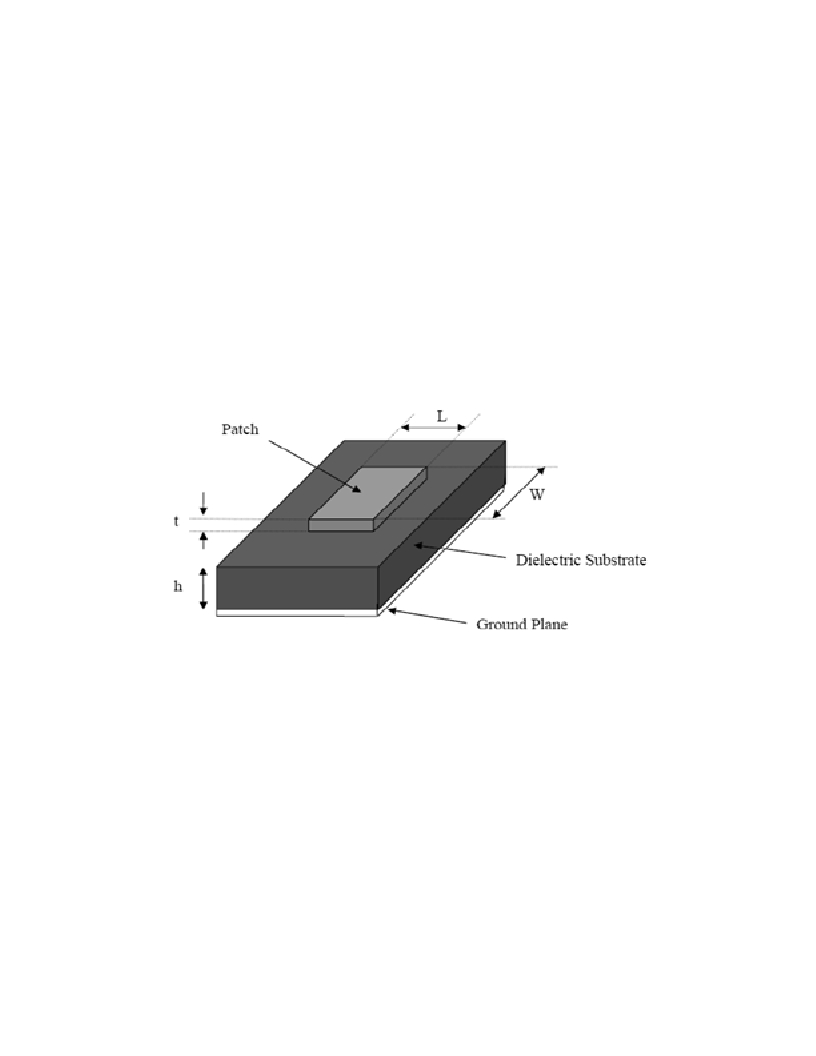
\includegraphics[height=3in]{/home/abc/Allprojects/project_report/System_Modelling/image1.png}
			 \caption{Basic Microstrip Patch Antenna}
		   \end{figure}

	  \justify
	   The electric field is zero at the center of the patch, maximum (positive) at one side, and minimum (negative) on the opposite side. It should be mentioned that the minimum and maximum continuously change side according to the instantaneous phase of the applied signal. The electric field does not stop abruptly at the patch's periphery as in a cavity rather, the fields extend the outer periphery to some degree. These field extensions are known as fringing fields and cause the patch to radiate. Some popular analytic modeling techniques for patch antennas are based on this leaky cavity concept. Therefore, the fundamental mode of a rectangular patch is often denoted using cavity theory as the TM10 mode.
	 \justify
	   Since this notation frequently causes confusion, we will briefly explain it. TM stands for transversal  magnetic field distribution. This means that only three field components are considered instead of six. The field components of interest are: the electric field in the z direction, and the magnetic field components in x and y direction using a Cartesian coordinate system, where the x and y axes are parallel with the ground plane and the z axis is perpendicular. In general, the modes are designated as TMnmz. The z value is mostly omitted since the electric field variation is considered negligible in the z axis. Hence TMmn remains with n and m the field variations in x and y direction. The field variation in the y direction (impedance width direction) is negligible; thus m is 0. And the field has one minimum to maximum variation in the x direction (resonance length direction); thus n is 1 in the case of the fundamental. Hence the notation TM10.

  \subsubsection{Dimensions}\label{sub:Dimensions}
	   \justify
	    The resonant length determines the resonant frequency and is about l/2 for a rectangular patch excited in its fundamental mode. The patch is, in fact, electrically a bit larger than its physical dimensions due to the fringing fields. The deviation between electrical and physical size is mainly dependent on the PC board thickness and dielectric constant.
	    A better approximation for the resonant length is:
	   \justify
	    This formula includes a first order correction for the edge extension due to the fringing fields, with:
	     \begin{itemize}
	       \item   L = resonant length
	       \item   λd = wavelength in PC board
	       \item λd = wavelength in PC board
	       \item λo = wavelength in free space
	       \item εr = dielectric constant of the PC board material

	     \end{itemize}

	     Other parameters that will influence the resonant frequency:

	     \begin{itemize}
	       \item Ground plane size
	       \item Metal (copper) thickness
	       \item  Patch (impedance) width
	     \end{itemize}

    \subsubsection{Impedance Matching}\label{sub:Impedance Matching}
     \justify
      Looking at the current (magnetic field) and voltage (electrical field) variation along the  patch, the current is maximal at the center and minimal near the left and right edges, while the electrical field is zero in the center and maximal near the left and minimal near the right edges.  The figures below clarify these quantities.

      % Here id figure
         \begin{figure}[h]
         	\centering
	         	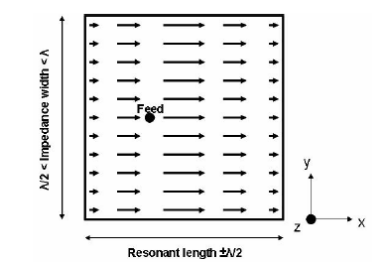
\includegraphics[height=3in]{/home/abc/Allprojects/project_report/System_Modelling/image2.png}
	         	\caption{Current Distribution On The Patch Surface}
         \end{figure}


	 \justify
      From the magnitude of the current and the voltage, we can conclude the impedance is minimum (theoretically zero W) in the middle of the patch and maximum (typically around 200W, but depending on the Q of the leaky cavity) near the edges. Put differently, there is a point where the impedance is 50 W somewhere along the "resonant length" (x) axis of the element.

        \begin{figure}[H]
         	\centering
           	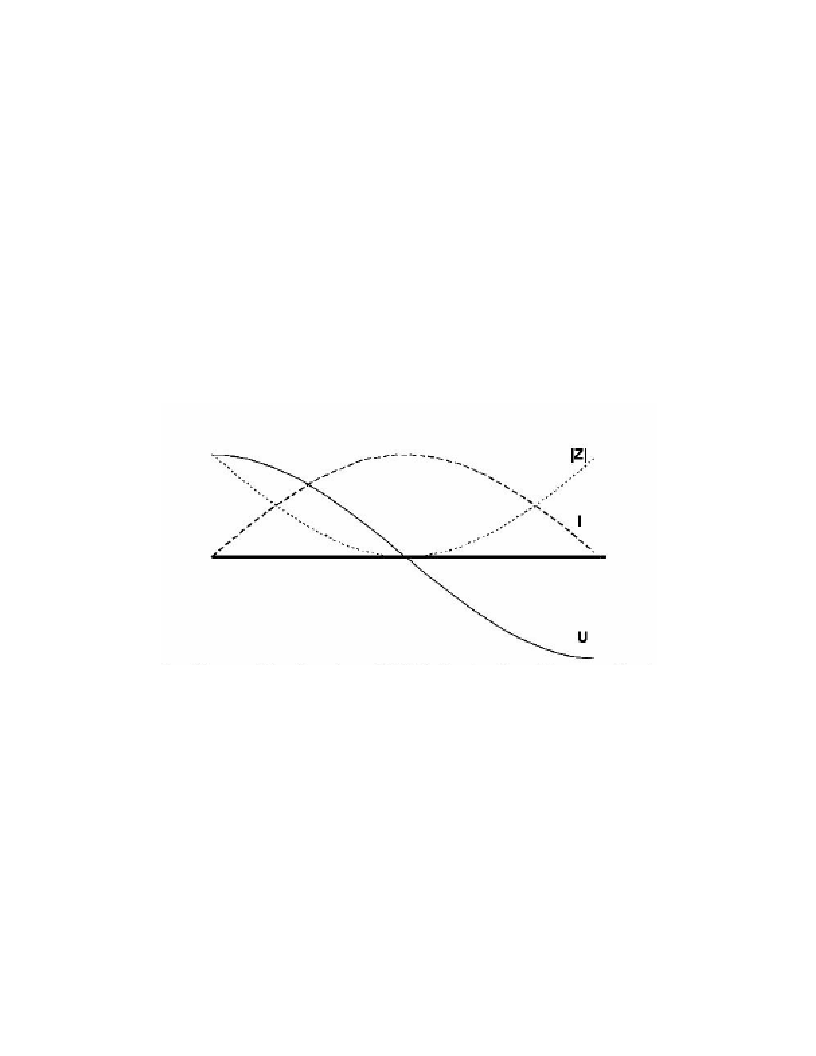
\includegraphics[height=3in]{/home/abc/Allprojects/project_report/System_Modelling/image3.png}
           	\caption{Voltage (V), Current (I), Impedance (Z ) Distribution along the Patch Resonant Length}
         \end{figure}



      \subsubsection{Radiation Pattern}
       \justify
        The patch's radiation at the fringing fields results in a certain far field radiation pattern. This radiation pattern shows that the antenna radiates more power in a certain direction than another direction. The antenna is said to have certain directivity. This is commonly expressed in dB .An estimation of the expected directivity of a patch can be derived with ease. The fringing fields at the radiating edges can be viewed as two radiating slots placed above a ground plane. Assuming all radiation occurs in one half of the hemisphere, this results in a 3 dB directivity.


        \begin{figure}[H]
        	\centering
        	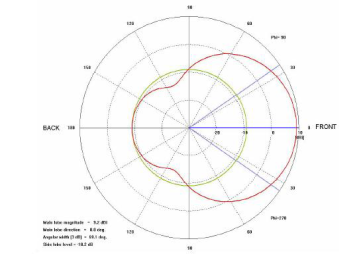
\includegraphics[height=3in]{/home/abc/Allprojects/project_report/System_Modelling/image4.png}
        	\caption{Typical Radiation Pattern of A Square Patch}
        \end{figure}

        This case is often described as a perfect front to back ratio; all radiation towards the front and no radiation towards the back. This front to back ratio is highly dependent on ground plane size and shape in practical cases. Another 3 dB can be added since there are 2 slots. The slots are typically taken to have a length equal to the impedance width (length according to the y axis) of the patch and a width equal to the substrate height. Such a slot typically has a gain of about 2 to 3 dB .This results in a total gain of 8 to 9 dB.

         The rectangular patch excited in its fundamental mode has a maximum directivity in the direction perpendicular to the patch (broadside). The directivity decreases when moving away from broadside towards lower elevations. The 3 dB beam width (or angular width) is twice the angle with respect to the angle of the maximum directivity, where this directivity has rolled off 3 16 dB with respect to the maximum directivity. An example of a radiation pattern can be found below. So far, the directivity has been defined with respect to an isotropic source and hence has the unit dBi. An isotropic source radiates an equal amount of power in every direction. Quite often, the antenna directivity is specified with respect to the directivity of a dipole. The  directivity of a dipole is 2.15 dBi with respect to an isotropic source. The directivity expressed with respect to the directivity of a dipole has dBd as its unit.

        \subsubsection{Antenna Gain}
         \justify

	        Antenna gain relates the intensity of an antenna in a given direction to the intensity that would be produced by a hypothetical ideal antenna that radiates equally in all directions or isotropically and has no losses. Since the radiation intensity from a lossless isotropic antenna equals the power into the antenna divided by a solid angle of 4π ste radians, we can write the following equation:\newline \newline

	        $ Gain= 4 \pi (Radition Intensity / Antenna InputPower right ) $
			\newline \newline

	        The gain of a rectangular Microstrip patch antenna with air dielectric can be very roughly Estimated as follows. Since the length of the patch, half a wavelength, is about the same as the length of a resonant dipole, we get about 2 dB of gain from the directivity relative to the vertical axis of the patch. If the patch is square, the pattern in the horizontal plane will be directional, somewhat as if the patch were a pair of dipoles separated by a half-wave; this counts for about another 2-3 dB. Finally, the addition of the ground plane cuts off most or all radiation behind the antenna, reducing the power averaged over all directions by a factor of 2 (and thus increasing the gain by 3 dB). Adding this all up, we get about 7-9 dB for a square patch, in good agreement with more sophisticated approaches.

        \subsubsection{Return Loss}\label{Return Loss}
		 \justify
          Return loss or reflection loss is the reflection of signal power from the insertion of a device in a transmission line or optical fiber. It is expressed as ratio in dB relative to the transmitted signal power.
          The return loss is given by: \newline \newline
          % formula
          $RldB = \log⁡(\rho {r} / \rho i)$

	      Where $\rho i $  is the power supplied by the source and $\rho r $ is the power reflected.


          \subsubsection{Polarization}\label{sub:Polarization}
           \justify
            The plane wherein the electric field varies is also known as the polarization plane. The
            basic patch covered until now is linearly polarized since the electric field only varies in one
            direction. This polarization can be either vertical or horizontal depending on the orientation of the patch. A transmit antenna needs a receiving antenna with the same polarization for optimum operation. The patch mentioned yields horizontal polarization, as shown. When the antenna is rotated 90°, the current flows in the vertical plane, and is then vertically polarized. A large number of applications, including satellite communication, have trouble with linear polarization because the orientation of the antennas is variable or unknown. Luckily, there is another kind of polarization circular polarization. In a circular polarized antenna, the electric field varies in two orthogonal planes (x and y direction) with the same magnitude and a 90° phase difference. The result is the simultaneous excitation of two modes, i.e. the TM10 mode (mode in the x direction) and the TM01 (mode in the y direction). One of the modes is excited with a 90° phase delay with respect to the other mode. A circular polarized antenna can either be right hand circular polarized (RHCP) or left-hand circular polarized (LHCP). The antenna is RHCP when the phases are 0° and 90° for the antenna in the figure below when it radiates towards the reader, and it is LHCP when the phases are 0° and 90°.

            \subsubsection{Bandwidth}
			 \justify
              Another important parameter of any antenna is the bandwidth it covers. Only impedance bandwidth is specified most of the time. However, it is important to realize that several definitions of bandwidth exist impedance bandwidth, directivity bandwidth, polarization bandwidth, and efficiency bandwidth. Directivity and efficiency are often combined as gain bandwidth.

             \subsubsection{Voltage Standing Wave Ratio}
              \justify
                This is the frequency range wherein the structure has a usable bandwidth compared to a certain impedance, usually 50 Ω. The impedance bandwidth depends on a large number of parameters related to the patch antenna element itself (e.g., quality factor) and the type of feed used. The plot below shows the return loss of a patch antenna and indicates the return loss bandwidth at the desired S11/VSWR (S11 wanted/VSWR wanted). The bandwidth is typically  limited to a few percent. This is the major disadvantage of basic patch antennas.

              \begin{figure}[H]
              	\centering
              	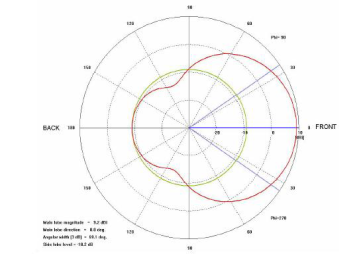
\includegraphics[height=3in]{/home/abc/Allprojects/project_report/System_Modelling/image4.png}
              	\caption{VSWR Bandwidth Calculation}
              \end{figure}


              \begin{itemize}
					\item
					Directivity/gain bandwidth
					This is the frequency range where in the antenna meets a certain directivity/gain
					requirement (e.g. 1 dB gain flatness).
					\item
					Efficiency bandwidth
					This is the frequency range wherein the antenna has reasonable (application dependent)
					radiation/total efficiency.
					16
					\item
					Polarization bandwidth
					This is the frequency range wherein the antenna maintains its polarization.

              \end{itemize}
			\cleardoublepage
              \subsubsection{Resonant Frequency}\label{sub:Resonant Frequency}
               \justify
	              The resonance frequency for the (1, 0) mode is given by
			          \newline    \newline
			          \centering
			              $ f_0 = C/2Le\sqrt{\epsilon_r } $

	               Where c is the speed of light in vacuum. To account for the fringing of the cavity fields at the edges of the patch, the length, the effective length Le is chosen as
	               \newline
						               \centering
	                                        Le= L + 2ΔL

	               The Hammerstad formula for the fringing extension is

	                 \begin{figure}[H]
	                 	\centering
	                 	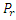
\includegraphics{/home/abc/Allprojects/project_report/System_Modelling/image6.png}

	                 \end{figure}

	                      Width of metallic patch (W)
				        \begin{figure}[H]
				        	\centering
				        	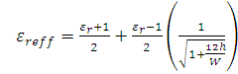
\includegraphics{/home/abc/Allprojects/project_report/System_Modelling/image7.png}

				        \end{figure}

                  Where,
                  \item
                    εreff = Effective dielectric constant
                    \item
                    εr = Dielectric constant of substrate
                  \item
                    h = Height of dielectric substrate
                     \item
                    W = Width of the patch

	         \cleardoublepage
				\subsection{Substrates }\label{sub:Substrates Characteristics}
		           \justify
		            There are many substrates that can be used for the design of microstrip antennas, and their dielectric constants (Er) are usually in the range of 2.2 $<$ Er $<$ 12. Thick substrates are most desirable for antenna performance as their dielectric constants are in the lower end, which provide better efficiency, larger bandwidth, loosely bound fields for radiation into space (better radiation power). However, these are achieved at the expense of larger element size, increase in weight, dielectric loss, surface wave loss and extraneous radiations. Thin substrates with higher dielectric constants, on the other hand, are desirable for microwave circuitry because they require tightly bound fields to minimize undesired radiation and coupling, thus leading to smaller sizes. However, because of their greater losses, they are less efficient and have relatively smaller bandwidth . Since microstrip antennas are often integrated with other microwave circuitry, a compromise has to be reached between good antenna performance and circuit design.

		            \begin{center}
		            	\begin{table}[H]
		            		\centering
		            		\begin{tabular}{ |l|l|}
		            			\hline
		            			Thick substrate &	Thin substrate \\ \hline
		            			Low dielectric constant & High dielectric constant  \\ \hline
		            			Better efficiency &	Less efficiency  \\ \hline
		            			Larger bandwidth &	Smaller bandwidth  \\ \hline
		            			Larger element size & Smaller element size  \\ \hline
		            			Increase in weight &	Lighter in weight  \\ \hline
		            			Increase in dielectric loss &	Minimum dielectric loss  \\ \hline


		            		\end{tabular}
		            				            	\caption{Table Thick and Thin  Substrate }
		            	\end{table}

		            \end{center}

	           \subsubsection{High Frequency Structure Simulator }
	            \justify
	                HFSS (High Frequency Structure Simulator) software is the industry-standard simulation tool for 3-D full-wave electromagnetic field simulation and is essential for the design of high-frequency and high-speed component design. This software automatically divides the geometric model into a large number of tetrahedron, where a single tetrahedron is a four-sided pyramid. This collection of tetrahedron is referred to as the finite element mesh. Each element can contain a different material. Therefore, the interface between two different materials must coincide with element boundaries. The value of a vector field quantity (such as the H-field or E-field) at points inside each tetrahedron is interpolated from the vertices of the tetrahedron. By representing field quantities in this way, the system can transform Maxwell's equations into matrix equations that are solved using traditional numerical methods. With HFSS, engineers can extract scattering matrix parameters (S, Y, Z parameters); visualize 3-D electromagnetic fields (near- and far-field).

	             \subsubsection{FR-4 Substrate}
		           \justify
		            FR-4 substrate is a very common and by far the most used substrate in consumer electronics market as it has a good quality-to-price ratio. It is mostly used where cost is more efficient than performance. FR-4 is a standard with many different distributors making many different FR-4 quality and property boards. It is made of woven fiber glass with an epoxy resin binder (binds the copper clad to the dielectric substrate) that is flame resistant.The dielectric constant goes down the more the FR-4 PCB is reinforced with epoxy resin instead of fiber glass as this is not determined as a standardized parameter. 100 \% epoxy resin boards has a dielectric constant of 3.4 @ 1MHz.
		           \justify
		           	The FR-4 changes it’s dielectric constant along its area which makes it too unstable to mass produce precise antennas on it. Also, the FR-4 is has a higher loss at frequencies over 3GHz, because of the sensitivity of the cheap substrate. Other products are therefore recommended to perform better than FR-4 in RF applications. A highly recommended distributor is Rogers, who is a little more expensive but performs much better in RF applications. In the cellphone industry, companies uses higher quality FR-4 substrate because it is more cost efficient, but from only one manufacture so they can be sure of the quality and properties when mass producing. The performance is typically around -13 dBm.\\

		            \begin{figure}[H]
		            	\centering
		            	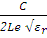
\includegraphics{/home/abc/Allprojects/project_report/System_Modelling/image8.png}
		            	\caption{Copper clad FR-4 PCB substrate.}
		            \end{figure}


\subsubsection{PCB Fabrication}
\justify
Various techniques are available for fabrication of micro strip patch antenna. If the substrate is flexible, conformal antennas are possible. Feed line and matching networks are fabricated along with antenna structure. The fabrication of strip antenna was designed using Auto CAD. Etching is done with the standard photolithographic processes. In order to transfer the mask image on electro plated copper PCB board photolithography technique was used. The cut size pieces of PCB sheets were cleaned to the surface impurities using organic solvents and then dried with hot air gun before coating the positive photo resist (PPR) on it. The PPR coated substrate was pre-baked in an oven at 90 degrees to remove the solvent and stuffing the film. The baked substrate was exposed on indigenously developed mask aligner with inbuilt exposure system and mask as prepared earlier . The accuracy of etching process also ensures uniformity of different parts over a production run.

\cleardoublepage
\subsubsection{ Testing of Antenna}
\justify
After Fabrication the antenna is tested for measurement of VSWR and return loss. As this project is based with only one datasheet of surface mounted device component so, it will obtain the desired result for the above parameter. The antenna parameter VSWR and Return loss is tested using Network Analyzer. Network analyzers incorporate new technologies and features to provide better performance and capabilities for antenna.

\begin{itemize}
	\item High sensitivity
	\item Fast data transfers with COM/DCOM
	\item LAN connectivity
	\item Flexibility and accuracy
	\item Pulsed measurements
	\item Security
\end{itemize}
\cleardoublepage
\subsection{Study of Different Gain and Bandwidth Enhancement Techniques}
\justify
The impedance frequency bandwidth of a microstrip antenna depends primarily on both the thickness and the dielectric permittivity of the substrate. A thick substrate with a low dielectric permittivity can increase the bandwidth of the printed patch. Both these selections could be a solution of the problem of bandwidth enhancement if the thickness of the substrate did not - cause difficulties in integration of the antenna with other microwave circuits, and  bcause some other problems such as the surface wave propagation and the large inductive image part of the input impedance of the antenna, which makes its resonance unfeasible.
  \subsubsection{ Substrate Selection}
   \justify
    The impedance frequency bandwidth of a microstrip antenna depends primarily on both the thickness and the dielectric permittivity of the substrate. A thick substrate with a low dielectric permittivity can increase the bandwidth of the printed patch. Both these selections could be a solution of the problem of bandwidth enhancement if the thickness of the substrate did not - cause difficulties in integration of the antenna with other microwave circuits, and  bcause some other problems such as the surface wave propagation and the large inductive image part of the input impedance of the antenna, which makes its resonance unfeasible.\\
 \subsubsection{Modified Shape Patches}
   \justify
    The regular MSA configurations, such as rectangular and circular patches have been modified to rectangular ring and circular ring, to enhance the BW. The larger BW is because of a reduction in the quality factor Q of the patch resonator, which is due to less energy stored beneath the patch and higher radiation.\\
  \subsubsection{ Planar Multi-resonator Configurations}
      \justify
     The planar stagger–tuned coupled multiple resonators yield wide BW in the same way as in the case of multistage tuned circuits. Several configurations are available yielding BW of 5–25 \%. Various parasitic patches like narrow strips, shorted quarter-wavelength rectangular patches, and rectangular resonator patches have been gap-coupled to the central-fed rectangular patch .These planar multi-resonator configurations yield broad BW.
 \subsubsection{Multilayer Configurations}
  \justify
    In the multilayer configuration, two or more patches on different layers of the dielectric substrate are stacked on each other. Based on the coupling mechanism, these configurations are categorized as electromagnetically coupled or aperture-coupled MSA.
    Various direct-coupled multi-resonators are:
    \begin{itemize}
    	\item    RMSAs direct-coupled along radiating edges,
    	\item    RMSAs direct-coupled along non-radiating edges,
    \end{itemize}
  \subsubsection{Electromagnetically Coupled MSAs}
    \justify
      In the electromagnetically coupled MSA, one or more patches at the different dielectric layers are electromagnetically coupled to the feed line located at the bottom dielectric layer.
      Alternatively, one of the patches is fed by a coaxial probe and the other patch is electromagnetically coupled. Either the bottom or top patch is fed with a coaxial probe. The patches can be fabricated on different substrates, and accordingly the patch dimensions are to be optimized so that the resonance frequencies of the patches are close to each other to yield broad BW.
    \subsubsection{ Stacked Multi-resonator MSAs}
      \justify
        The planar and stacked multi-resonator techniques are combined to further increase the BW and gain. A probe-fed single rectangular or circular patch located on the bottom layer has been used to excite multiple rectangular or circular patches on the top layer, respectively. Besides increasing the BW, these configurations also provide an increase in gain as well. \\


          	Following are Different types of shapes embedded to enhance the BW and gain

        \begin{itemize}

        	\item Symmetric Rectangular slots
        	\item Two square slots
        	\item Symmetric trapezoidal slot
        	\item V-shaped slots
        	\item Shifted Elliptical Slot

        \end{itemize}
       \subsubsection{ Design of  Rectangular Patch Antenna for UWB Application}
        \justify
         The three essential parameters for the design of a rectangular Microstrip Patch Antenna, Frequency of operation (fo). The resonant frequency of the antenna must be selected appropriately. The Mobile Communication Systems uses the frequency range from 2100-5600 MHz. Hence the antenna designed must be able to operate in this frequency range. The lowest order mode TM01 resonates when the effective length of the rectangular patch is half wavelength. Radiation occurs from the fringing fields. For the principal E-plane, the dimensions of the patch along its length have been extended on each end by a distance ΔL, as show in Figure , which is a function of the effective dielectric constant and the width-to-height ratio (W/h).
          \begin{figure}
          	\centering
          	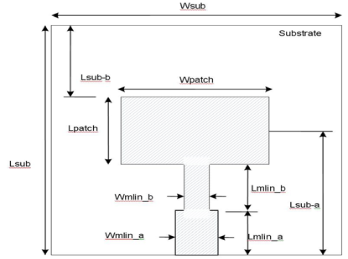
\includegraphics[height=3in]{/home/abc/Allprojects/project_report/System_Modelling/image9.png}
          	\caption{The design geometry ofthe proposed antenna patch UWB antenna.}
          \end{figure}

         Theoretical design:

         Step 1: Calculation of the Width (W):

         The width of the Microstrip patch antenna is given as:

         Where
             c - Free space velocity of light, 3 x 108 m/s
         fr - Frequency of operation
         εr - dielectric constant

         Step 2: Calculation of Effective dielectric constant (εreff):
         The effective dielectric constant is:

         Where;
                εr - Dielectric constant
         h - Height of dielectric substrate
         W - Width of the patch
         Step 3: Calculation of the Effective length (Leff):
         The effective length is:

         Where;
          c - Free space velocity of light, 3 x 108 m/s
         fr - frequency of operation
         εreff - effective dielectric constant

         Step 4: Calculation of actual length of patch (L):
         The actual length is obtained by:
         L = Leff - 2∆L
         Where,
         L 	= Actual length of patch.
         Leff 	 = Effective length.
         ∆L 	= small difference between length.

         Step 5: Calculation of the length extension (∆L):
         The length extension is:     24

         Figure shows the simple rectangular patch antenna.
         The length, L= 35mm,
         Width w= 45mm,
         Cut width= 10mm
         and cut width= 5mm,
         length of transmission line feed= 32mm,
         width of the feed= 3mm.
         The rectangular microstrip patch antenna designed on one side of the epoxy structure with εr = 4.4 and height from the ground plane= 1.6mm. \\



         The simulated peak gains and efficiencies of the antennas from 1 to 17 GHz . It can be seen that all of the antennas have almost the same gain and efficiency, so again the slots do not have much effects on the performances throughout the entire operation band. The average gains of these antennas from 3.1to 10.6 GHz are about 2.8 dBi and the average efficiencies are about 0.88

         \begin{center}
         		\begin{table}[H]
         			\centering
         			\begin{tabular}{ |l|l|}
         				\hline
         				Parameter & Specification \\ \hline
         				Patch Shape &  Plan rectangular patch \\ \hline
         				Frequency Range &  3.1–16.3 GHz \\ \hline
         				Dielectric constant of substrate & 4.4 \\ \hline
         				Height of substrate &   1.6mm \\ \hline
         				Feeding method &  Microstrip feed line \\ \hline
         				Polarization &  Circular \\ \hline
         			\end{tabular}
         			\caption{Design Parameter}
         		\end{table}
         \end{center}

        \subsubsection{Feed Techniques}
          \justify
           Microstrip patch antennas can be fed by a variety of methods. These methods can be
           classified into two categories- contacting and non-contacting. In the contacting method, the RF power is fed directly to the radiating patch using a connecting element such as a microstrip line. In the non-contacting scheme, electromagnetic field coupling is done to transfer power between the microstrip line and the radiating patch . The four most popular feed techniques used are the microstrip line, coaxial probe (both contacting schemes), aperture coupling and proximity coupling (both non-contacting schemes).

         \paragraph{ Microstrip Line Feed}
           \justify
            In this type of feed technique, a conducting strip is connected directly to the edge of the microstrip patch as shown in Figure 3.3. The conducting strip is smaller in width as compared to the patch and this kind of feed arrangement has the advantage that the feed can be etched on the same substrate to provide a planar structure.

            \begin{figure}[H]
            	\centering
            	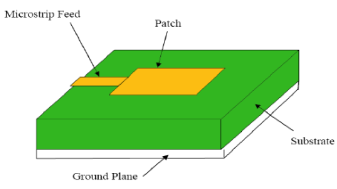
\includegraphics[height=3in]{/home/abc/Allprojects/project_report/System_Modelling/image10.png}
            	\caption{Microstrip Line Feed.}
            \end{figure}


         	The purpose of the inset cut in the patch is to match the impedance of the feed line to the patch without the need for any additional matching element. This is achieved by properlycontrolling the inset position. Hence this is an easy feeding scheme, since it provides ease of fabrication and simplicity in modeling as well as impedance matching. However as the thickness of the dielectric substrate being used, increases, surface waves and spurious feed radiation also increases, which hampers the bandwidth of the antenna . The feed radiation also leads to undesired cross polarized radiation
         \paragraph{ Coaxial Feed}
          \justify


            The Coaxial feed or probe feed is a very common technique used for feeding Microstrip patch antennas. As seen from Figure 3.4, the inner conductor of the coaxial connector extends through the dielectric and is soldered to the radiating patch, while the outer conductor is connected to the ground plane. The main advantage of this type of feeding scheme is that the feed can be placed at any desired location inside the patch in order to match with its input impedance.
               \begin{figure}[H]
               	\centering
               	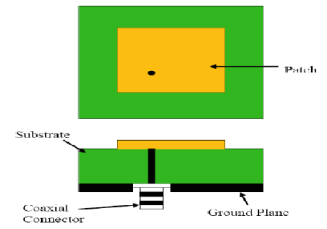
\includegraphics[height=3in]{/home/abc/Allprojects/project_report/System_Modelling/image11.png}
               	\caption{Probe feed Rectangular Microstrip Patch Antenna. }
               \end{figure}
             This feed method is easy to fabricate and has low spurious radiation. However, a major disadvantage is that it provides narrow bandwidth and is difficult to model since a hole has to be drilled in the substrate and the connector protrudes outside the ground plane, thus not making it completely planar for thick substrates (h > 0.02λo). Also, for thicker substrates, the increased probe length makes the input impedance more inductive, leading to matching problems . It is seen above that for a thick dielectric substrate, which provides broad bandwidth.


          \paragraph{Aperture Coupled Feed}
           \justify
            In this type of feed technique, the radiating patch and the microstrip feed line are separated by the ground plane as shown in Figure 2.5. Coupling between the patch and the feed line is made through a slot or an aperture in the ground plane.  The coupling aperture is usually centered under the patch, leading to lower cross-polarization due to symmetry of the configuration. The amount of coupling from the feed line to the patch is determined by the shape, size and location of the aperture.

              \begin{figure}[H]
              	\centering
              	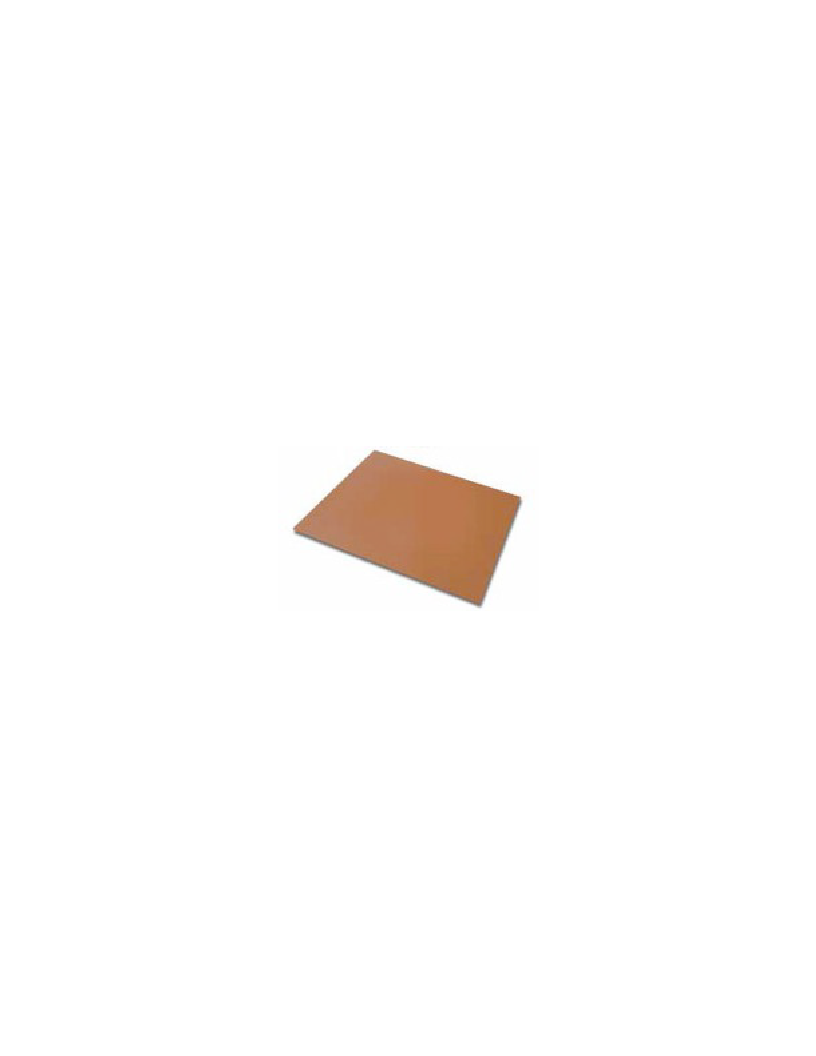
\includegraphics[height=3in]{/home/abc/Allprojects/project_report/System_Modelling/image12.png}
              	\caption{Aperture-coupled feed }
              \end{figure}

             Since the ground plane separates the patch and the feed line, spurious radiation is minimized. Generally, a high dielectric material is used for bottom substrate and a thick, low dielectric constant material is used for the top substrate to optimize radiation from the patch . The major disadvantage of this feed technique is that it is difficult to fabricate due to multiple layers, which also increases the antenna thickness. This feeding scheme also provides narrow bandwidth.

           \paragraph{ Proximity Coupled Feed}
            \justify
             This type of feed technique is also called as the electromagnetic coupling scheme two dielectric substrates are used such that the feed line is between the two substrates and the radiating patch is on top of the upper substrate. The main advantage of this feed technique is that it eliminates spurious feed radiation and provides very high bandwidth (as high as 13 \%) , due to overall increase in the thickness of the microstrip patch antenna. This scheme also provides choices between two different dielectric media, one for the patch and one for the feed line to optimize the individual.

         \subsection{ Basic Principles of Operation}
          \justify
           The  metallic  patch  essentially  creates  a  resonant  cavity,  where  the  patch  is  the  top  of  the cavity, the ground plane is the bottom of the cavity, and the edges of the patch form the sides of the cavity. The edges of the patch act approximately as an open-circuit boundary condition. Hence, the patch acts approximately as a cavity with perfect electric conductor on the top and bottom surfaces, and a perfect “magnetic conductor” on the sides. This point of view is very useful in analyzing the patch antenna, as well as in understanding its behavior. Inside the patch cavity the electric field is essentially z directed and independent of the z coordinate. Hence, the patch cavity modes are described by a double index (m, n). For the (m, n) cavity mode of the rectangular patch the electric field has the form

           Where L is the patch length and W is the patch width. The patch is usually operated in the (1,0) mode,  so  that  L  is  the  resonant  dimension,  and  the  field  is  essentially  constant  in  the y direction. The surface current on the bottom of the metal patch is then x directed, and is given by

           For  this  mode  the  patch  may  be  regarded  as  a  wide  microstrip  line  of  width  W,  having  a resonant  length  L  that  is  approximately  one-half  wavelength  in  the  dielectric.  The  current  is maximum  at  the  centre  of  the  patch,  x  =  L/2,  while  the  electric  field  is  maximum  at  the  two “radiating” edges x=0 and x=L. The width W is usually chosen to be larger than the length (W =1.5 L is typical) to maximize the bandwidth, since the bandwidth is proportional to the width. (The width should be kept less than twice the length, however, to avoid excitation of the (0, 2) mode .
           At first glance, it might appear that the Rectangular Microstrip Patch Antenna will not be an effective radiator when the substrate is electrically thin,   However, the Q of the cavity increases as  h decreases (the radiation Q is inversely proportional to h). Hence, the amplitude A10  of the modal field  at  resonance  is  inversely  proportional  to  h.

           Hence,  the  strength  of  the  radiated  field  from  a resonant patch is  essentially independent  of  h,  if  losses are ignored. The resonant input resistance will  likewise  be  nearly  independent  of  h.  This  explains  why  a  patch  antenna  can  be  an  effective radiator even for very thin substrates, although the bandwidth will be small.

          \begin{figure}[H]
          	\centering
          	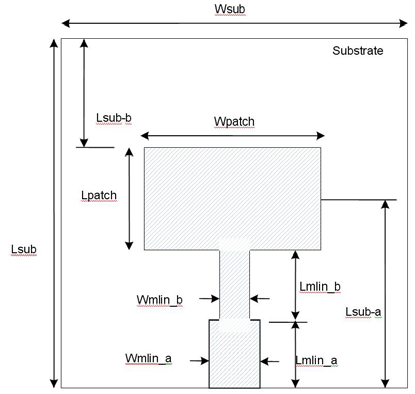
\includegraphics[height=3in]{/home/abc/Allprojects/project_report/System_Modelling/image13.png}
          	\caption{Common Shapes Of Microstrip Patch Elements}
          \end{figure}

           Microstrip patch antennas radiate primarily because of the fringing fields between the patch edge and the ground plane. For good antenna performance, a thick dielectric substrate having a low dielectric constant is desirable since this provides better efficiency, larger bandwidth and better radiation . However, such a configuration leads to a larger antenna size. In order to design a compact Microstrip patch antenna, substrates with higher dielectric constants must be used which are less efficient and result in narrower bandwidth. Hence a trade-off must be realized between the antenna dimensions and antenna performance.

          \cleardoublepage

           \section{Advantages and Application}
            \justify
             Microstrip patch antennas are mostly used in wireless applications due to their low profile Structure. Therefore they are extremely compatible for embedded antennas in handheld Wireless devices such as cellular phones, pagers etc.
             Some of the principal advantages are given below:
             \begin{itemize}
             	\item Light weight and less volume.
             	\item Low fabrication cost, therefore can be manufactured in large quantities.
             	\item Supports both, linear as well as circular polarization.
             	\item Low profile planar configuration which can be easily made conformal to host surface.
             	\item Can be easily integrated with microwave integrated circuits (MICs).
             	\item Capable of dual and triple frequency operations.
             	\item Mechanically robust when mounted on rough surfaces.
             \end{itemize}


             \subsection{Application}
             \begin{itemize}
             	\item Satellite communications
             	\item Microwave communications
             	\item Cell phone antennas
             	\item GPS antennas

             \end{itemize}


         	


\cleardoublepage

\section{Conclusion}\label{sec:Conclusion}
    \subsection{Energy, Economy Environment Aspect:}\label{sub:Energy, Economy Environment Aspect:}
       Multiband freq. band at 2GHz,3.06GHz  3.84GHz  .Slot shapes embedded along the four diagonal directions on the patch radiators gives circularly polarization. The proposed patch antenna will be designed using above designing parameters and the responses obtained using HFSS simulation software.
    \subsection{Project Planning:}\label{sub:Project Planning:}

    \subsection{Cost estimation:}\label{sub:Cost estimation:}
      The costing includes two dimensions
      a.  designing
      b. fabrication
      The designing includes more labour than monetary factors. Once the design is ready the antenna will be ready very early.  The fabrication of antenna in size is very small.  It is like two credit cards.
      The approximate cost will be near about 4 to 5 K.
\cleardoublepage

\section{ACKNOWLEDGEMENT}
  \justify
	It gives us a great pleasure to submit  Project report.This is the only page where we have the opportunity to express our emotions and gratitude . We express our sincere thanks to our guide \textbf{Mr. V.P.Kardile} sir for guiding us at every step in making of this project. He motivated us and boosted our confidence and We must admit that the work would not have been accomplished without his guidance and encouragement. \\


	We would like to extend our special thanks to \textbf{H.O.D Prof. V.M. Kulkarni} and \textbf{Principal Dr. J.H. Godihal} for spending their valuable time to go through our report and providing many helpful suggestions. Lastly We would like to thank all the staff member of electronics department and my friends without whom the project report would not have been completed.\\


	 \begin{flushright}
	 	Amol Dhormare(.....................) \\
	 	Abhishek Joshi(....................) \\
	 	Rushank Deshpande(...................) \\
	 	B.E. (Electronics and communication Engineering) \\
	 \end{flushright}




\end{document}
